\graphicspath{{content/summary/figures/}}

\section{Privire de ansamblu}

Teza fa't'a va introduce un nou utilitar care poate rezolva automat
condi'tii de curs'a 'in programe Java. Exist'a dou'a fapte relevante
ale ingineriei software care stau la baza motiva'tiei utilitarului:

%This thesis will introduce a new tool that can automatically fix
%data-races in Java programs. There are two relevant facts of software
%engineering that will help the reader better understand the motivation behind
%the tool:
\begin{enumerate}
  \item inginerii software au trebuit s'a 'tin'a 'in fr\aa u cele mai
  complexe sisteme construite de om 'in ultimele decenii
  %software engineers have had to manage, arguably, the most complex
  %systems ever built by humans for decades now.
  
  \item comunitatea de dezvoltare software s-a bazat pe legea lui Moore pentru
  a-i ajuta cu 'imbun'at'a'tirea performan'tei software-ului scris 'inc'a
  de la bun 'inceput. Dar ast'azi, accentul 'in 'imbun'at'a'tirea
  performan'tei hardware a trecut de la cre'sterea vitezei de procesare a
  CPU-urilor la integrarea a mai multora, care lucreaz'a 'in paralel, pe
  acela'si chip
  %the software development community has been relying on Moore's Law
  %to help improve the performance of their software since its beginning. But
  %nowadays hardware performance boosting has shifted from higher CPU speed
  %towards multiple processing units working in parallel.
\end{enumerate}

Pentru a putea m\aa nui complexit'a'tile men'tionate mai sus, programatorii au
dezvoltat o multitudine de metode; una dintre ele find \emph{refactorizarea}
(transformare efectuat'a asupra codului care 'ii las'a neschimbat
comportamentul ini'tial). \^In ani recen'ti multe din aceste refactoriz'ari au
fost automatizate 'si marea parte a IDE-urilor ofer'a un mod de utilizare u'sor
pentru programator, 'in special pentru cod scris 'in Java. Automatizarea
refactoriz'arilor relev'a un concept interesant: separarea rolurilor din cadrul
interac'tiunii ma'sin'a-om. Omul este responsabil de men'tinerea consisten'tei
modelului abstract, de nivel 'inalt al sistemului; 'in timp ce ma'sina execut'a
analizele 'si transform'arile greoaie 'si repetitive necesare finaliz'arii unei
refactoriz'ari.
%In order to handle the above mentioned complexity programmers have developed
% numerous methods to help cope with it, one of which is \emph{refactoring}
% (behaviour preserving transformations performed on the code). In recent years
% many of these refactorings have been automated and all major IDEs offer
% user-friendly support for these transformations, especially for code written in
% the Java language. The automation of refactorings, in turn, reveals an
% interesting concept: the separation of roles in human-machine interaction.The
% human is responsible for the consistency of the abstract, high-level concerns of
% the system, while the machine performs the tedious and repetitive analyses and
% transformations necessary for performing refactorings.

'In plus, dificult'a'tile ridicate de 'incercarea de a rula cod 'in paralel,
\emph{'in mod corect}, nu sunt triviale; adaug'a acest lucru la simplul fapt c'a
software-ul standard este, 'in sinea lui, foarte greu de 'tinut 'in fr\aa u, 'si
aducerea software-ului deja existent c'atre noua paradigm'a multi-core devine o
problem'a foarte dificil'a. Una dintre cele mai des 'int\aa lnite probleme
legat'a de execu'tia 'in paralel sunt condi'tiile de curs'a. O condi'tie de
curs'a apare atunci c'and dou'a fire de execu'tie 'incearc'a s'a acceseze
acelea'si date 'in acela'si timp, unul cu un acces de citire, cel'alalt cu unul
de scriere.
% Furthermore, the difficulties raised by trying to make code execute
% \emph{correctly} in parallel are non-trivial; add this to the fact that
% standard software systems are in of themselves hard to manage, retrofitting
% old software to this new paradigm becomes a very difficult problem. One of the
% most common issue in parallel programs are data races; a data race arises when
% two different threads contend for the same data, one with a write access the
% other one with a read access.

\paragraph{Din cele enun'tate mai sus} o idee destul de evident'a poate veni
'in minte: un utilitar care ar ajuta programatorul s'a transforme cod executat
secven'tial 'in cod paralel; astfel, u'sur\aa nd povara programatorului de a
trebui s'a efectueze transform'ari greoaie pe sistemele mo'stenite a c'aror
performan't'a nu mai scaleaz'a cu hardware-ul nou. Un astfel de utilitar deja
exist'a 'si se nume'ste ReLooper~\cite{ReLooper}. Pe scurt, ReLooper prime'ste
ca date de intrare un ciclu care efectueaz'a calcule de lung'a durat'a pe seturi
largi de date 'si 'il transform'a folosind structura de date \emph{ParalelArray}
oferit'a de Java, care faciliteaz'a execu'tia convenient'a pe elementele unui
tablou a task-urilor paralele. Aceast'a transformare poate fi efectuat'a numai
dac'a execu'tia acestor task-uri nu rezult'a 'intr-un \emph{data-race} 'in contextul
executiei paralele.
% \paragraph{From the two points above}an obvious idea comes to mind: a tool that
% helps the programmer transform sequential code into parallel code; thus
% freeing the programmer from the burden of the tedious transformations done on
% legacy systems whose performance no longer improves with new hardware.
% Such a tool exists in the form of ReLooper\cite{ReLooper}. Briefly described,
% ReLooper takes as input a user-selected loop that performs computationaly intensive
% operations on large data sets and converts it using Java's \emph{ParalelArray}
% data structure which facilitates easy execution of parallel tasks on the array's
% elements. This transformation can be performed only if the code that comprises
% these tasks does not result in any data-races in the context of parallel execution.

\paragraph{Utilitarul nostru} vine ca o extensie natural'a pentru ReLooper
datorit'a faptului c'a 'incearc'a s'a rezolve astfel de condi'tii de curs'a.
Dar, acestea se pot manifesta 'in feluri multiple. Ca urmare, noi am recurs la o
bun'a practic'a 'in proiectarea utilitarelor automatizate de refactorizare, 'si
anume: identificarea celor mai comune transform'ari f'acute pe sistemele
software din lumea real'a pentru a putea avea un adev'arat impact asupra
productivit'a'tii programatorului. A'sadar, am 'inceput cu analizarea a 34 de
proiecte Java open-source (dintre care 3 au fost candida'ti viabili pentru
paralelizare). Am observat c'a trebuia s'a efectu'am acea'si schimbare 'in mod
repetat; adic'a, transformarea datelor care erau partajate de fire de execu'tie
'in a'sa fel 'inc\aa t fiecare fir s'a aib'a propria lui copie a datelor.
Exist'a dou'a metode prin care se poate realiza acest lucru:
% \paragraph{Our tool}comes as a natural extension to ReLooper in the sense that
% it attempts to solve such data-races. But, data-races can manifest themselves
% in multiple ways so we used a best practice when it comes to automated
% refactoring tools: identifying the most common changes that are executed in a
% consistent manner in real world software systems, in order have the greatest
% impact on programmer productivity. Thus, we started out by analyzing a total
% of 34 open-source Java projects (out of which 3 were viable candidates for
% parallelization). We realized that we had to make one particular change over
% and over again. Namely, make data that was once shared between threads unique
% to each one; every thread getting its own copy of the data. There are two ways
% of doing this:
\begin{enumerate}
  \item [a)] mutarea aloc'arii obiectelor 'in contextul paralel. Determinarea,
  prin analiz'a static'a, dac'a acest lucru este posibil nu este o problem'a
  trivial'a.
  \item [b)] 'incapsularea obiectelor 'in \emph{ThreadLocal}-ul oferit de Java,
  o clas'a 'inf'a'sur'a-toare care asigur'a c'a fiecare fir are access la
  instan'te unice a datelor.  Un program secven'tial executat cu obiecte
  \emph{ThreadLocal} se comport'a la fel ca 'si versiunea veche, dar 'si
  garanteaz'a c'a atunci c'and este executat 'in paralel fiecare fir
  prime'ste propria copie a datelor, totul pentru un cost suplimentar de
  execu'tie. Pentru a ar'ata c'a acest cost nu este neglijabil am f'acut
  urmatoarele: 'in cazul programului Jmol~\cite{Jmol-site}, pur 'si simplu
  am refactorizat fiecare c\aa mp care era victima unui data-race (34 de c\aa
  mpuri 'in total) 'in \emph{ThreadLocal}. Diferen'ta 'in performan't'a este
  de la 1.4s (media de rulare secven'tial) la 2.2s; a'sadar un cost de
  aproximativ 63\% 'in performan't'a.
\end{enumerate}

% \begin{enumerate} 
%   \item [a)] move object allocation to the parallel context. Identify whether or
%   not this is possible is a non-trivial problem. 
%   \item [b)] encapsulate objects in Java's \emph{ThreadLocal}, a wrapper class
%   that ensures that the data enclosed is unique for each thread. A sequential
%   program executed using \emph{ThreadLocal} objects behaves the same as the old
%   version, but it also ensures that when executed concurrently each thread
%   receives its own copy of the data, all at the cost of some overhead
%   introduced by \emph{ThreadLocal} itself. To show that this overhead is not
%   negligible we did the following: in the case of Jmol\cite{Jmol-site}, we
%   simply refactored each individual field that was involved in a race (34
%   fields) to be \emph{ThreadLocal}. The difference in performance is from an
%   average sequential running time of 1.4s to 2.2s; so an overhead of roughly
%   63\%.
% \end{enumerate}

O privire de ansamblu a tuturor task-urilor computa'tionale efectuate de
utilitarul nostru pentru a putea aplica transformarile de mai sus pot fi
v'azute 'in figura~\ref{algo}. Acestea vor fi explicate ulterior.

% An abstract overview of the major computational tasks that our tool does in
% order to perform the above mentioned transformation can be seen in
% Figure~\ref{algo}.

\begin{figure}[h!]
\begin{center}
  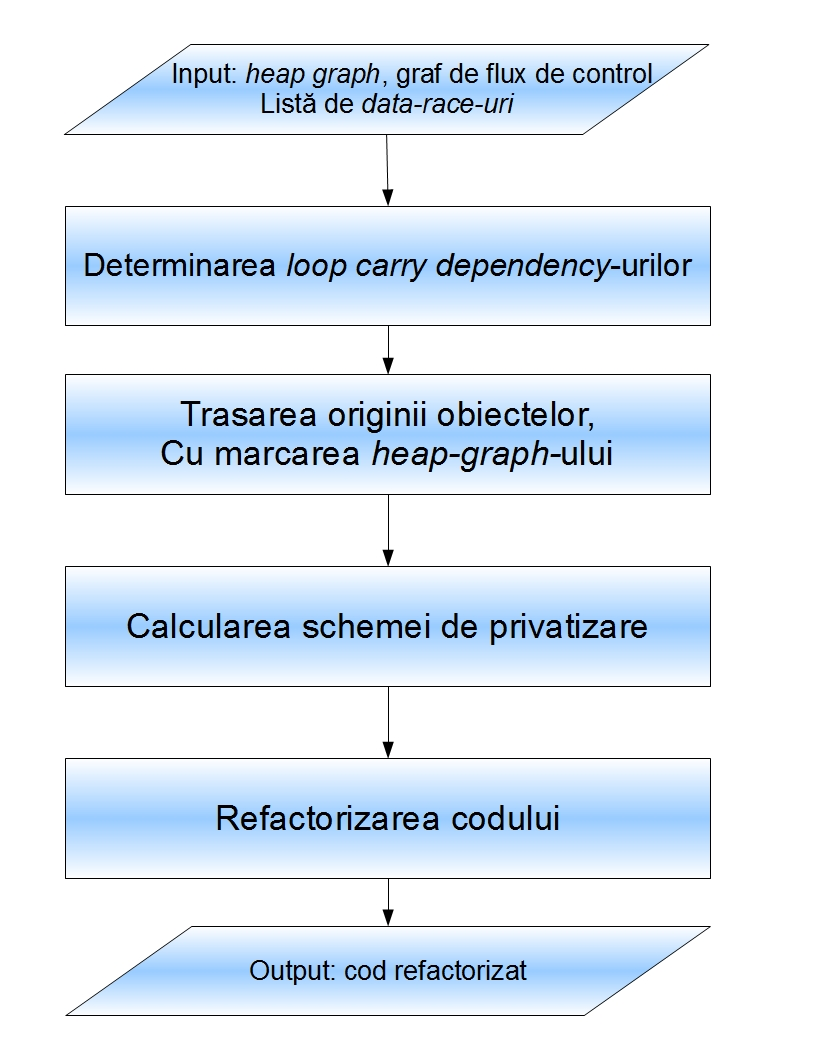
\includegraphics[width=7cm]{algo}
  \caption{Schema logic'a a algoritmului}
  \label{algo}
\end{center}
\end{figure}

Noi am denumit clasa de transformari mentionate mai sus drept \emph{privatizarea
datelor}, care va fi 'si termenul folosit de noi de acum 'incolo. Aceast'a
lucrare se va concentra asupra metodei \emph{b)} de privatizare, dar cu mici
varia'tii. 'In loc de \emph{ThreadLocal} noi folosim propria noastr'a clasa
numit'a \emph{ThreadPrivate} care se comport'a 'in mare parte ca 'si
\emph{ThreadLocal}, dar ofera suport robust pentru garantarea faptului c'a
datele referite 'in fiecare fir sunt 'in starea corect'a (adic'a starea de
dinaintea 'inceperii contextului paralel).
% We dubbed the transformations described above as \emph{data privatization},
% which will be the term we will use hereafter. This thesis will focus mostly on
% the second method, but with slight variations. Instead of \emph{ThreadLocal}
% we use our own construct called \emph{ThreadPrivate} which behaves mostly like
% \emph{ThreadLocal}, but it offers more robust support for ensuring that the
% copy of the data that is referenced in each of the threads is in the proper
% state (i.e. the one it is in right before the execution of the parallel
% operation).

\paragraph{O precondi'tie foarte important'a} care trebuie 'indeplinit'a este ca
datele s'a nu fie parte dintr-o clas'a special'a de \emph{data-race}-uri pe care
noi le numim \emph{dependin't'a 'intre itera'tiile ciclului}. 'In principiu c\aa
mpurile nu au voie s'a fie folosite ca 'si tampon temporar 'intre itera'tiile
ciclului. Determinarea cu 'incredere a faptlui c'a un data-race este sau nu un
\emph{loop carried dependency} s-a dovedit a fi cea mai dificil'a problem'a
'int\aa mpinat'a de noi 'in timpul dezvoltarii acestui utilitar. Necesit'a o
analiz'a complex'a a grafului de flux de control ob'tinut prin analiza statica a
codului Java.
Din pricina faptului ca determinarea de \emph{loop carried dependency}-uri a fost
la vremea respectiv'a o problem'a nerezolvat'a a trebuit s'a trecem prin c\aa
teva 'incerc'ari nereu'site p\aa n'a c'and ne-am dat seama c'a ea face parte din
clasa problemelor \emph{interprocedural, finite, distributive, subset (IFDS)}.
Din fericire, WALA~\cite{wala-site}, biblioteca de analiz'a static'a pe care o
folosim ofer'a suport pentru astfel de probleme; ca urmare, am reu'sit s'a
invent'am o solu'tie elegant'a 'si compact'a care func'tioneaz'a 'in 100\%
dintre cazuri, 'in compara'tie cu solu'tiile anterioare care erau imprecise 'si
mult mai complicate.

% \paragraph{A very important} precondition that has to be met is that the data is
% not involved in a particular type of data-race that we call a \emph{loop carry
% dependency}. Basically the fields must not be used as temporary storage between
% the iterations of the loop. Reliably determining whether or not a data-race is
% a \emph{loop carried dependency} has proven to be the most challenging task in
% building this tool. It requires a complex analysis of the control flow graph
% obtained through static analysis of the Java source code.
% Because of the fact that the detection of loop carry dependencies was at that
% point in time an unsolved problem we've had to go through several failed
% attempts before we've concluded that it is basically an \emph{interprocedural,
% finite, distributive, subset (IFDS) problem}~\cite{IFDS}. Luckily, WALA
%~\cite{wala-site}, the static analysis library we used offered support for
% solving these kinds of problems and we came up with a very elegant and compact
% solution that works with 100\% accuracy; as opposed to the previously verbose
% and inaccurate solutions.

\paragraph{Dupa determinarea} c\aa mpurilor ce pot fi privatizate 'in
siguran't'a le c'aut'am originea. Rue'sim acest lucru printr-un algoritm care
traverseaz'a \emph{heap graph}-ul prin urmarirea \emph{def-use}-urilor a c\aa
mpului 'in cauz'a. Urm'arirea este limitat'a la contextul operatorului paralel
de ciclu deoarece pe noi ne intereseaz'a ultimul proprietar al obiectului la
'inceputul opera'tiei paralele. Acest ultim proprietar va fi 'tinta
refactoriz'arii.
% \paragraph{After determining} which of the fields can be safely privatized we
% trace their origin. We do that using a graph algorithm that traverses the heap
% graph by going through the def-uses of the field in question. The trace is
% limited to the context of the parallel loop operator because we care only about
% the last owner of the objects at the start of the parallel context. This last
% owner is the one that will be the target of the refactoring.

\paragraph{'In cele din urma,} informa'tiile adunate 'in timpul tras'arii
orginii sunt folosite pentru a calcula ``schema`` de privatizare care are ca
scop minimizarea costului aditional introdus de \emph{ThreadPrivate}. Aceasta
``schema`` este folosit'a de refactorizarea noastr'a (dezvoltat'a ca o extensie
a IDE-ului eclipse) pentru a efectua schimb'arile necesare.

% \paragraph{Last,}the information gathered during the origin trace is used to
% compute the privatization scheme which aims to minimize the overhead introduced by
% \emph{ThreadPrivate}. This privatization scheme is used by our refactoring
% (built on top of the eclipse IDE) to perform the necessary transformations.

\section{Implementarea}
Marea parte a complexit'a'tii proiectului este una de natur'a teoretic'a, odat'a
ce am rezolvat aceste probleme, implementarea utilitarului a devenit
relativ simpl'a. Nu am 'int\aa mpinat dificult'a'ti inginere'sti notabile,
utilitarul nostru av\aa nd 6000 linii de cod distribuite prin 30 clase; iar
interac'tiunea dintre acestea este simpl'a 'si comprehensibil'a.
% \section{Implementation}
% The bulk of the complexity of our project was theoretical, once these issues
% have been solved the implementation of the tool itself becomes simple. We
% encountered no noteworthy engineering difficulties, our tool comprising of
% roughly 6000 lines of code distributed over 30 classes, the interaction between
% these is simple and very comprehensible.

Pentru a v'a da idee de cantitatea de efort depus 'in faza ini'tial'a 'in
care analizam proiecte open-source, pentru a realiza prima paralelizare manuala
a Jmol-ului a trebuit s'a:
\begin{itemize}
  \item rul'am programul cu utilitarul de profilare YourKit~\cite{YourKit}
  pentru a g'asii ciclurile cu intensitate computa'tional'a mare.
  \item analiz'am 101 c\aa mputi distribuite 'in 6 clase, care sunt referite de
  997 ori 'in contextul ce urma s'a devin'a paralel, pentru a determina dac'a
  sunt sau nu \emph{data-race}-uri
  \item privatiz'am cele 34 de c\aa mpuri care s-au dovedit a fi {data-race}-uri
  folosing \emph{ThreadLocal}
  \item privatizarea a necesitat schimbarea a 359 de referin'te la aceste c\aa
  mpuri datorit'a indirect'arii introduse de \emph{ThreadLocal}
\end{itemize}


% But to give you an idea on the of the amount of work we put into the initial
% phase of analysing open-source projects, to do the first manual parallelization
% of Jmol we had to:
% \begin{itemize}
%   \item run the program with a the YourKit Java profiler~\cite{YourKit}in order
%   to find computationally intensive loops.
%   \item analyze 101 fields distributed over 6 classes, that were reference a
%   total of 997 times in the future parallel context to check for data-races
%   \item privatize the 34 fields that were proven to be data-races using
%   \emph{ThreadLocal}
%   \item the privatization led the update of 359 field references due to the
%   indirection introduced by \emph{ThreadLocal}
% \end{itemize}
\section{Concluzii}

\paragraph{'In concluzie,} aceasta lucrare propune o solu'tie nou'a pentru o
problema des 'int\aa lnit'a 'in 'incercarea de a transforma cod secven'tial 'in
cod paralel. De asemenea, prezint'a un utilitar experimental care este 'in stare
s'a efectueze aceste transform'ari pe versiuni reduse a proiectelor analizate
(reduse la doar cateva zeci de mii de linii de cod). Dar solu'tia pentru
determinarea de \emph{loop carried dependency}-uri este, poten'tial, o contribu'tie
de folos viitoarelor utilitare de detec'tie a condi'tiilor de curs'a sau a
utilitarelor de verificare a corectitudinii executiei paralele.

% \section{Conclusions}
% 
% \paragraph{In conclusion,} this thesis proposes a novel solution for a fairly
% common problem encountered when trying to retrofit sequential code to parallel
% code and it presents an experimental tool that is able to successfully perform
% these transformations on sandbox versions of the analyzed projects (i.e.
% reduced programs to only a few tens of thousands of lines of code). But the
% novel theoretical issue of determining loop carry dependencies is,
% potentially, a useful contribution to future race-detection or parallel
% correctness verification tools.
